\documentclass{beamer}

\usepackage[utf8]{inputenc}
\usepackage{graphicx}
\usepackage{booktabs}
\graphicspath{ {./Figures/} }

\title{Predictive modelling of alcohol-associated risks in College students}
\author{Olivier Binette and Raphael Morsomme}
\date{February 18, 2020}

\begin{document}

\frame{\titlepage}

\begin{frame} \frametitle{Goals}

\textbf{Develop a predictive model of alcohol related risks} in college students using information readily available to schools, in order to help:

\begin{enumerate}
  \item identify students at risk and allocate support ressources as effectively as possible;
  \item determine if additional information could help identify students at risk.
\end{enumerate}

\textbf{Assumption:} alcohol-related risks are an important issue that a school wants to address on its own through supporting students in need.
  
\end{frame}


\begin{frame} \frametitle{Challenges}

What we deal with:

\begin{enumerate}
  \item \textbf{Meaningfulness.} We predict a ``student need'' score which is a function of student awareness and alcohol-related risks.
  \item \textbf{Reliability.} We provide interval predictions with exact frequentist coverage. This communicates uncertainty in the prediction and could help mitigate issues related to over-confidence in the model.
\end{enumerate}

\end{frame}

\begin{frame} \frametitle{Challenges}

Things we don't deal with (but that we should):

\begin{enumerate}
  \item \textbf{Interpretability.} It is difficult to summarize the model and explain the predictions.
  \item \textbf{Fairness.} Non-discrimination (title IX). Issues using race, gender, age as predictors. Suitability of the ``student need'' response across these groups and quality of the data among them.
  \item \textbf{Side effects.} We globally care about student well-being and success, not just about alcohol-related risks. Depending on how the model is used, only focusing on alcohol could have adverse effects on other issues.
  \item \textbf{Data representativeness.} The data may not represent a given school's student population and post-stratification would be necessary.
\end{enumerate}

\end{frame}


\begin{frame} \frametitle{Response variable}



\end{frame}


\begin{frame} \frametitle{Is it worth it?}


\begin{itemize}
	\item Predictive model to identify students at risk of alcohol-related issues
	\item Consider two nested sets of predictors
	\begin{itemize}
		\item variables that the school already has e.g. age and sex
		\item variables that the school could easily collect e.g. religion and marital status of parents additional predictors
	\end{itemize}
	\item Compare the predictive power of the two models using the \textit{conformal prediction} framework.
\end{itemize}
\end{frame}


\begin{frame} \frametitle{Response Variable}

Three measures of risk:
\begin{itemize}
	\item behavioral risk
	\item ...
\end{itemize}

Construct the response variable with the following formula
$$\text{Risk}_i = X_i + y_i * z_i ^ \pi$$

\end{frame}


\begin{frame} \frametitle{Conformal Predictors}

Prediction intervals that are
\begin{itemize}
	\item valid at a given significance level for \textit{finite} sample (Vovk, 2005)
	\item distribution-free
	\item universal
	\item individualized (Papadopoulos, 2009)
	\item only assume exchangeability
	\item cheap (Papadopoulos, 2002)
\end{itemize}
\end{frame}


\begin{frame} \frametitle{Inductive Conformal Prediction}

Given a labeled training set $\{z_i = (x_i, y_i)\}_{i=1}^n$ and an unlabeled test observation $x_{n+1}$,
\begin{enumerate}
	\item partition training set into a \textit{proper training} set $\{z_j\}_{j=1}^l$ and a \textit{calibration} set $\{z_k \}_{k=l+1}^n$
	\item fit predictive model on proper training set
	\item compute predictions $\hat{y}_k$ on calibration set and anomaly scores
	$$a(z_k) = |\hat{y}_k - y_k|, \quad k = l+1, \dots, n$$
	\item identify $a_\epsilon$, the $\epsilon^{\text{th}}$ percentile of the $\{a\}_{k=l+1}^n$
	\item compute prediction on test observation and set the prediction interval to be
	$$\{y: |\hat{y}_{n+1} - y| < a_\epsilon\}$$
	\end{enumerate}
\end{frame}


\begin{frame} \frametitle{Set up}
\begin{itemize}
	\item Test set is $10\%$ of data set
	\item Calibration set is $30\%$ of training set.
	\item Repeat $100$ times to obtain the expected width of prediction intervals	
	\item Predictive model: Random Forest with $1,500$ trees, $m = p/3$ and default pruning.
\end{itemize}
\end{frame}

\begin{frame} \frametitle{Results - Coverage}  
% latex table generated in R 3.5.2 by xtable 1.8-3 package
% Mon Feb 17 15:58:32 2020
\begin{table}[ht]
\centering
\begin{tabular}{rrlrr}
  \toprule
 & Significance & Set of Predictors & Mean Width & Coverage \\ 
  \midrule
1 & 0.500 & Extensive & 1.138 & 0.503 \\ 
  2 & 0.500 & Restricted & 1.370 & 0.501 \\ 
  3 & 0.750 & Extensive & 1.807 & 0.754 \\ 
  4 & 0.750 & Restricted & 2.109 & 0.749 \\ 
  5 & 0.900 & Extensive & 2.513 & 0.909 \\ 
  6 & 0.900 & Restricted & 2.801 & 0.897 \\ 
  7 & 0.950 & Extensive & 2.896 & 0.954 \\ 
  8 & 0.950 & Restricted & 3.212 & 0.951 \\ 
   \bottomrule
\end{tabular}
\caption{Coverage and Mean Width of Prediction Intervals} 
\end{table}

\end{frame}

\begin{frame} \frametitle{Results - Width}   
\begin{figure}
	\centering
	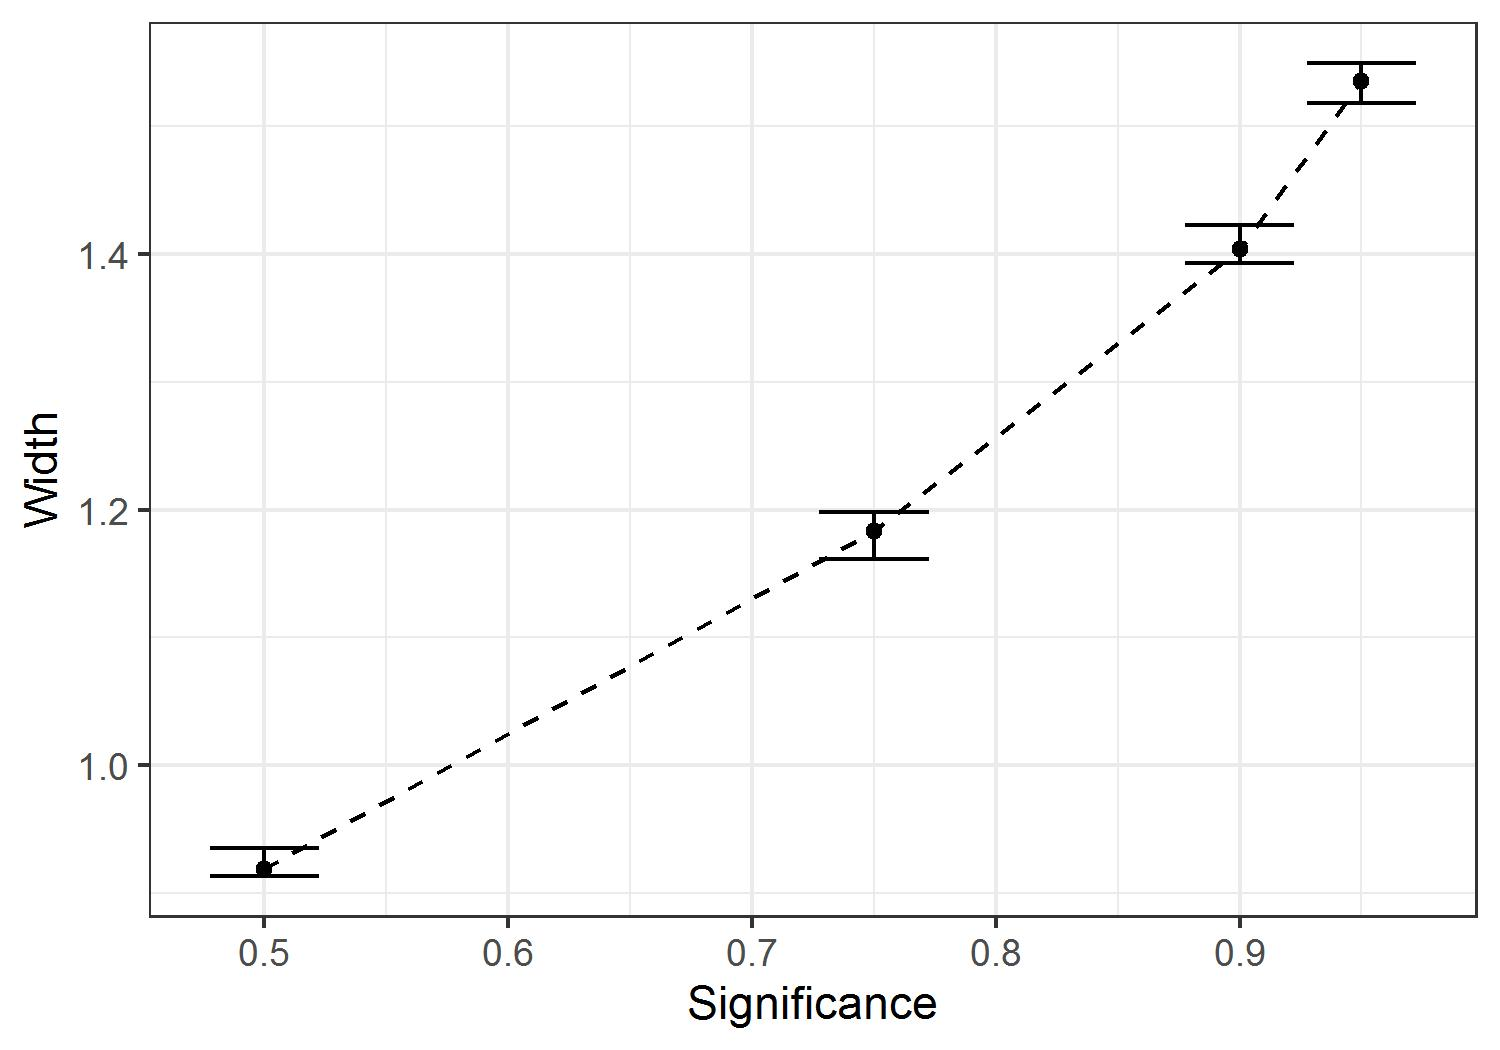
\includegraphics[scale = 0.5]{conformal.jpeg}
	\caption{Median and inter-decile interval width across significance levels.}
	\label{fig:conformal}
\end{figure}
\end{frame}

\begin{frame}
Future directions
\begin{itemize}
	\item tune the pruning of the trees in the RF
\end{itemize}
\end{frame}





\begin{frame}
\frametitle{References}
\footnotesize{
	\begin{thebibliography}{99} % Beamer does not support BibTeX so references must be inserted manually as below
		
		\bibitem[Vovk, 2005]{Whickam2009} Vovk, A. \\
		\newblock Tidy Data\\
		\newblock \emph{Journal}, month year
		
		\bibitem[Papadopoulos, 2002]{Valente2005} Valente, j. \\
		\newblock Apartment Rent Prediction Using Spatial Modeling\\
		\newblock \emph{Journal}, month year
		
		\bibitem[Papadopoulos, 2009]{Belasco2012} Belasco, E. \\
		\newblock Using a Finite Mixture Model of Heterogeneous Households to Delineate Housing Submarkets\\
		\newblock \emph{Journal}, month year
		
	\end{thebibliography}
}
\end{frame}
    






\end{document}
